%%%%%%%%%%%%%%%%%%%%%%%%%%%%%%%%%%%
\subsection{Front-end Readout and Buffering}
\label{sec:fd-daq-fero}

\metainfo{Giles Barr \& Giovanna Miotto \& Brett Viren, this is DP-specific.  This file is \texttt{far-detector-dual-phase/chapter-fddp-daq/design-fero.tex}}

\begin{dunefigure}[\dual \dword{fe} \dword{daq} fragment]{fig:daq-readout-buffering-baseline}
  {Illustration of data (solid arrows) and trigger (dashed) flow for
    two \dual \dword{fe} \dword{daq} fragments. 
    One servicing eight of \num{240} \dword{cro} crates and the other servicing all
    five \dword{lro} crates.  
    Black arrows indicate nominal flow and red indicate special flow
    for handling of potential \dword{snb}.} 
    %See text for detail description.}
  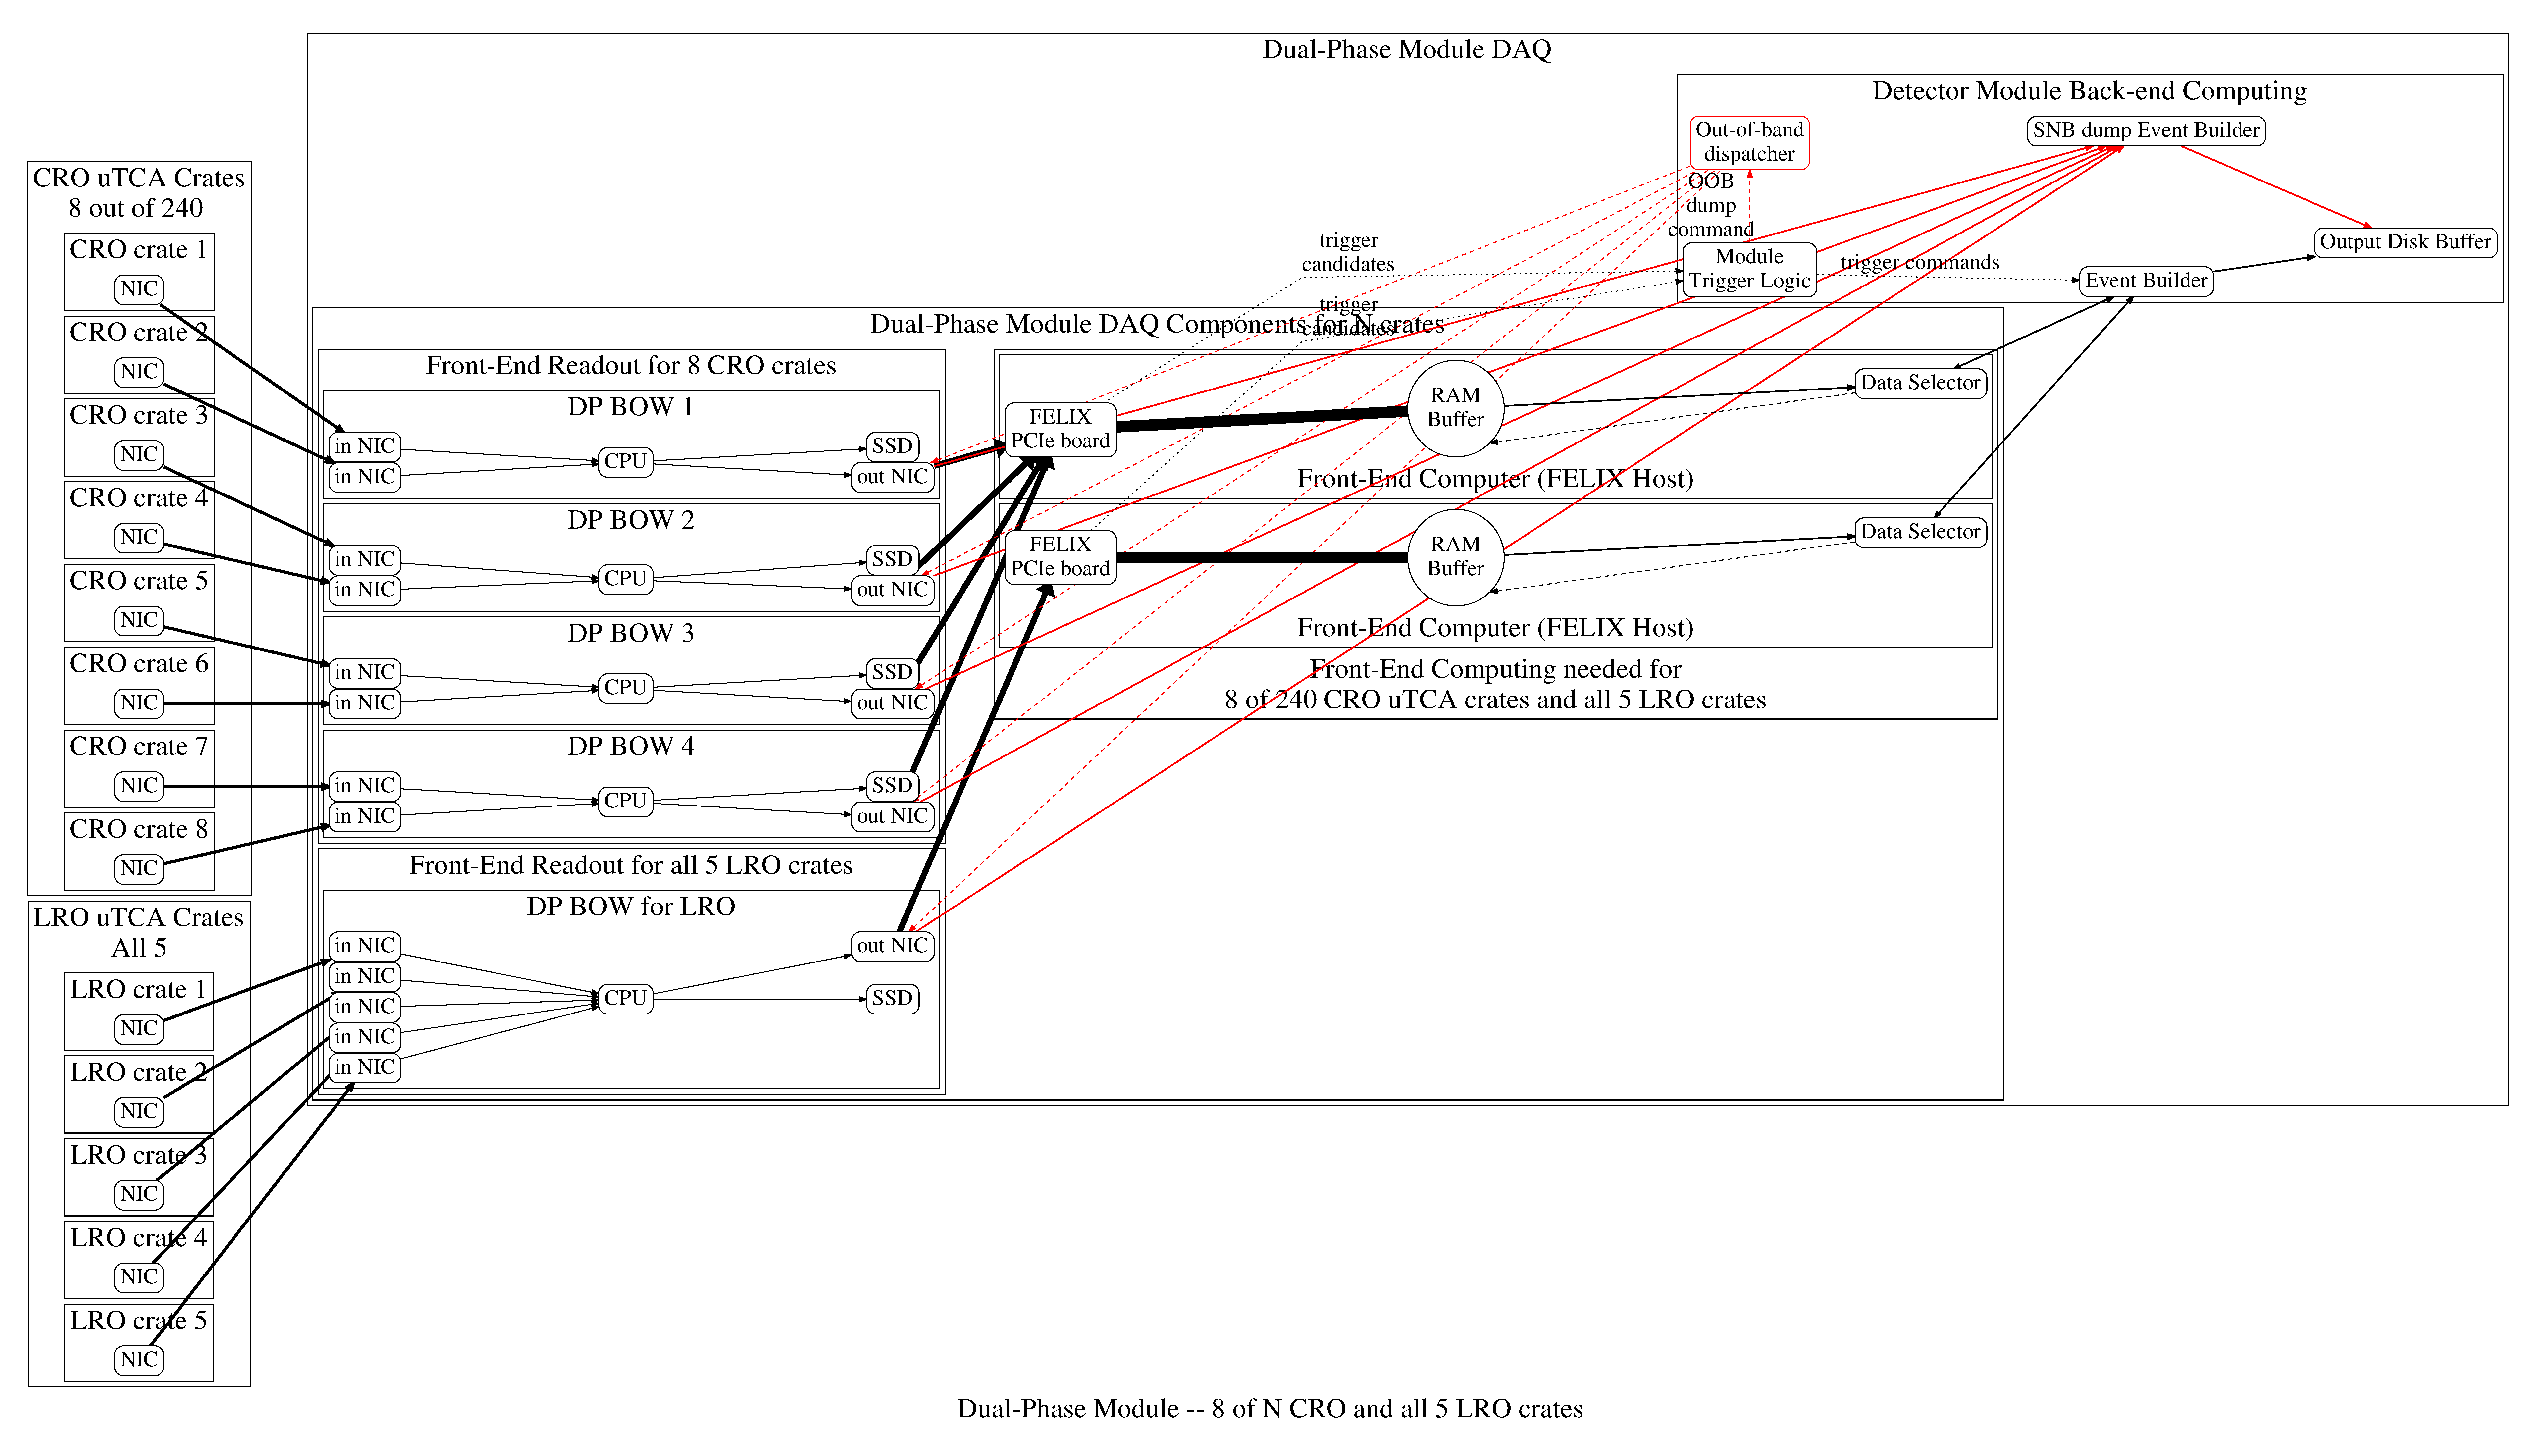
\includegraphics[width=0.95\textwidth,clip,trim=1cm 0 1cm 0]{daq-readout-buffering-baseline.pdf}%
\end{dunefigure}

Figurere~\ref{fig:daq-readout-buffering-baseline} illustrates
\dual-specific implementation of the nominal, generic \dword{daq} front-end
\dword{daqfrag} design shown in Figure~\ref{fig:daq-overview}. 
The \dword{cro} crates deliver data on \dword{udp} to \dword{bow} computers
which implement the \dword{daqfer} duties.
The \dword{cro} data is delivered to the \dword{daq} \dword{bow} computers with lossless
compression applied and so before the \dwords{trigprimitive} can be
produced the data must be decompressed. 

In order to save on cost, power, space, cooling, etc., a number of \dword{cro}
crate data streams can be aggregated into one \dword{fec}. 
The \dword{cro} data stream is sent using \dword{udp} which is not expected to provide
reliable transport of high-throughput data if a network switch
intervenes. 
Thus each \dword{cro} requires a corresponding \SI{10}{\Gbps} \dword{nic} in the receiving
\dword{bow} computer.
With the expected 10$\times$ lossless compression factor the nominal
output from each \dword{cro} crate will be \SI{2}{Gbps}. 
If noise levels are higher than expected the throughput will increase,
however even very noisy data should be compressible enough to fit into
the \SI{10}{Gbps} bandwidth. 
Noise will be better understood from \dword{pddp} data, and studies
are needed to optimize the number of \dword{cro} crates per \dword{bow}
computer.

After processing, the input data is sent out, along with the
corresponding primitives to a \dword{felix} board in a \dword{fec}. 
Similar to the argument above about noise, bandwidth and \dword{bow} computer
multiplicity, the number of \dword{bow} data streams that can be aggregated
into each \dword{felix} board requires additional study. 
The current generation of \dword{felix} boards have been tested with a
throughput to system RAM of \SI{10}{\GB/\s}. 
The next generation is expected to at least double that. 
With the caveat that these tests did not receive data on \dword{udp}, a nominal
\SI{20}{\GB/\s} throughput is assumed possible for the next-generation
PCIe v4 boards. 
Given this assumption and that the expected noise levels are achieved,
then based solely on bandwidth, as many as \num{80} \dword{cro} data streams might be
aggregated into a single next-generation \dword{felix} board. 
Figure~\ref{fig:daq-readout-buffering-baseline} indicates the
aggregation of eight \dword{cro} streams, which represents the multiplicity
required to deal with very high noise. 
Future studies are needed to determine %understand 
which of these two extremes to favor for optimization of the design,
%the design may be optimized toward 
but the basic design itself is
fairly elastic between them.

The \dword{lro} crates are nominally not involved in self-triggering although
the data from all five \dword{lro} crates are assumed to flow through a \dword{lro} \dword{bow}. 
%This includes data from all five \dword{lro} crates; 
The data are then sent to a
single \dword{felix} board. 
Given the expected data rates, that \dword{felix} board must ingest about
\SI{25}{\GB/\s}.

The second duty of the \dword{daqfer} in the nominal design is to
provide non-volatile storage for receiving full-stream data dumps when
an \dword{snb} dump trigger command is issued. 
With today's technology, individual \dwords{ssd} can write at about \SI{2.5}{GB/s}. 
Up to four \dwords{ssd} have been placed on a \num{1}-lane PCIe v3 board and have
achieved about three times this speed. 
This would allow an individual \dword{bow} computer to aggregate \numrange{10}{30} \dword{cro}
data streams before the \dwords{ssd} become a bottleneck. 
The five \dword{lro} data streams, each producing \SI{5}{Gbps}, could together be
streamed to a two modern \dwords{ssd}. %\fixme{??}
The \dword{bow} computers must also have sufficient RAM to hold
pre-\dword{snb}-trigger data of about \num{10} seconds.

The alternative design (not diagrammed), which corresponds to
Figure~\ref{fig:daq-overview-alt}, deletes the layer containing \dword{bow}
computers and directly connects the \dword{udp} streams from the \dword{cro} and \dword{lro}
crates to the \dword{felix} boards in the \dwords{fec}. 
The \dword{cro} (compressed) data is buffered on the \dword{felix} host computer RAM
and distributed to the trigger farm for decompression and \dword{trigprimitive} and \dword{trigcandidate} processing. 
The remaining part of the \dword{trigdecision} is as in the nominal
design except that the \dword{snb} dump data stream is handled symmetrically
with the normal triggered data.
